%==========================================================================
%Template File for Evolutionary Computation Symposium
%==========================================================================
\documentclass[a4paper,11pt,twocolumn]{jarticle}
\usepackage{evocomp}
\usepackage{fancyhdr}
\usepackage[linesnumbered,ruled]{algorithm2e}
\usepackage{graphicx}
\usepackage{subcaption}
\usepackage[table,dvipsnames]{xcolor}% http://ctan.org/pkg/xcolor
\def\doubleunderline#1{\underline{\underline{#1}}}

% Declares special characters to be used in equations:
\newcommand{\B}{{\mathbb{B}}}
\newcommand{\I}{{\mathbb{I}}}
\newcommand{\E}{{\mathbb{E}}}
\newcommand{\R}{{\mathbb{R}}}
\newcommand{\Rnn}{{\mathbb{R}_+}}           % { x ∈ R ∣ x ≥ 0 }
\newcommand{\Rp}{{\mathbb{R}_+^*}}          % { x ∈ R ∣ x > 0 }
\newcommand{\N}{{\mathbb{N}}}
\newcommand{\Np}{{\mathbb{N}_+^*}}          % { x ∈ N ∣ x > 0 }

\pagestyle{empty}

\renewcommand{\headrulewidth}{0.0pt}
\renewcommand{\footrulewidth}{0.0pt}

\renewcommand\refname{References}

\begin{document}
\twocolumn[%
\begin{center}

\beginheader

\jtitle%
{Error-Driven Ranking for Evolutionary-Computing Estimation of Nash Equilibria in Simultaneous Continuous Games}

\begin{authors}
\name{1}{Rui Leite},
\name{1}{Hernan Aguirre},
\name{2}{Gilberto Reynoso-Meza},
\end{authors}



\begin{affiliation}
\aff{1}{Shinshu University},
\aff{2}{Pontifícia Universidade Católica do Paraná (PUCPR)},
\end{affiliation}

\endheader

\end{center}
]

\etitle{Error-Driven Ranking for Evolutionary-Computing Estimation of Nash Equilibria in Simultaneous Continuous Games}

\ename{1}{Rui Leite(23hs201j@shinshu-u.ac.jp)}
\ename{1}{Hernan Aguirre(ahernan@shinshu-u.ac.jp)}
\ename{2}{Gilberto Reynoso-Meza(g.reynosomeza@pucpr.br)}

\eaff{1}{%
Shinshu University
}
\eaff{2}{%
Pontifícia Universidade Católica do Paraná (PUCPR)
}

\vspace{3mm}

\kanjiskip=.1zw plus 3pt minus 3pt
\xkanjiskip=.1zw plus 3pt minus 3pt

% Abstract (200 words max.)
% Game theory has recently gained attention in the field of cybersecurity, as it provides a formal framework to model the interactions between attackers and defenders.
% In this context, the solution concept of Nash equilibrium is often used to identify optimal strategies for all players concurrently.
% For games of simultaneous decision and continuous strategy sets with an infinite number of Nash equilibria, producing an accurate and diversified set of estimations for such equilibria is a challenging task.
% In this work, we present a novel ranking scheme meant for evolutionary algorithms that approximate Nash equilibria for simultaneous continuous games with multi-objective players.
% The proposed ranking procedure leverages information from previous generations to guide the search towards high-quality solutions, while still encouraging diversity by avoiding a hyper-focus on optimizing fitness values alone.
% We conducted experiments with a cybersecurity game model called FlipIt with Infrastructure Enhancement, which has an infinite number of Nash equilibria.
% The results show that the proposed approach is competitive with existing methods, being particularly effective in terms of solution diversity and hardware usage.

\section{Introduction}

Advanced Persistent Threats are sophisticated, long-term cyberattacks where adversaries infiltrate a computer infrastructure and remain undetected for extended periods, aiming to steal sensitive data or cause significant damage.
They led to a shift in cybersecurity paradigms, emphasizing the importance of proactive defense strategies that assume that breaches might occur undetected.
In this context, game theory has been increasingly applied to model the interactions between attackers and defenders.
FlipIt \cite{dijk2013flipit} is a prominent example of such a game-theoretical model, specifically designed to capture the dynamics of stealthy cyberattacks and defenses with the intent of improving cybersecurity policies.

The goal of game-theoretical analysis is to find the Nash Equilibria (NE) of the game.
NE are states where all players successfully maximize their payoffs given the strategies of the other players, and are often considered ``game solutions'' \cite{bonanno2018game}.
A game is not a pure Multi-Objective Optimization Problem (MOOP), as the players are not cooperating towards a common global optimum.
Games require dedicated solution methods, since each player controls some of the decision variables, and all decisions influence all players' outcomes.
In situations like this, conflicts are likely to arise.

FlipIt with Infrastructure Enhancement (IE) \cite{leite2024cec} is an extension of FlipIt that incorporates multi-objective players and continuous strategy spaces, enabling more complex models that better reflect real-world cyber scenarios.
Finding NE via algebra in these cases gets increasingly complicated with the complexity.
This is why numerical methods are often preferred.
Co-Evolutionary Algorithms (CoEA) were used for estimating solutions for FlipIt with IE by evolving populations of decision-variable values concurrently \cite{leite2024cec}.
This approach led to very accurate approximations, but presented challenges in terms of architectural complexity and diversity of estimations.
Another work \cite{leite2024jpnsec} proposed a novel evolutionary-computing based optimization procedure for continuous games of simultaneous decision, specifically aimed at providing a more comprehensive framework for approximating game solutions by decomposing the decision space into a grid of MOOPs.
This framework generalizes the basic analytical methods from game theory and leverages concepts of evolutionary computation to transform an otherwise infinite problem into a finite set of optimization ones; however, the computational cost grows non-linearly with the grid resolution.
Finally, in \cite{leite2025gecco} a simpler CoEA architecture was proposed that searches for a single NE per run, incorporating special requirements to ensure future applicability in a coordinating process to find multiple equilibria in a single run.

In this paper, we propose a novel evolutionary algorithm ranking scheme for solving game-theorical models of simultaneous decision, continuous decision spaces, and any number of players and solutions.
The ranking procedure is based on the continuous patching of individual ranks over generations, instead of instantaneous fitness relations between individuals.
This method was designed to achieve a good balance between computational efficiency and solution diversity.

The remainder of this paper is organized as follows: Section \ref{relatedworks} reviews related works; Section \ref{algorithm} describes the proposed method; Section \ref{methodology} presents the experimental setup; Section \ref{results} discusses our findings; and Section \ref{conclusions} concludes with potential avenues for future research.


\section{Related Works}
\label{relatedworks}


\subsection{Game Theory and Nash Equilibria}
\label{gametheory}

Games where decisions are taken simultaneously by all players can be modeled by a quadruple $\left (I, (S_0, S_1, \dots, S_{n-1}), O, f \right )$ \cite{bonanno2018game}.
$I = \{0, 1, \dots, n-1\}$ is a list of player identifiers (where $n \geq 2$ is the number of players).
$S_p$ is player $p$'s strategy set (with $p \in I$), that is, the set of all possible decisions that player $p$ can take.
$O$ is the set of possible outcomes, and $f: S \rightarrow O$ is the payoff function, where $S = S_0 \times S_1 \times \dots \times S_{n-1}$.
In game theory, a strategy profile is a tuple $s \in S$ of game decisions by all players that defines a complete game scenario.
The basic solution for such games is the Pure-Strategy Nash Equilibria (PSNE) \cite{bonanno2018game}, defined here as a subset $E \subseteq S$ comprised of each strategy profile $s^* = (s^*_0, s^*_1, \dots, s^*_{n-1})$ such that:

\vskip-15pt
\begin{equation*}
    \forall{p} \forall{s_p}~ f(s^*) \succeq_p f(s^*_0, \dots, s^*_{p-1}, s_p, s^*_{p+1}, \dots, s^*_{n-1})
\end{equation*}

\noindent
where each $s_p \in S_p$ and each $s^*_p \in S_p$, and $\succeq_p$ is a relation such that $f(a) \succeq_p f(b)$ denotes that $p$'s perceived outcome from $a$ is preferred to that of $b$.

Nash equilibria reflect the choices that rational players could take, and are thus often seen as ``solutions'' to a game model, as long as the players are aware of the game dynamics and the model properly incorporates players' preferences.
For finite games, the PSNE can usually be found analytically by basically evaluating all possible strategy profiles exhaustively.
For games with continuous strategy sets, however, this is not feasible, and numerical methods are used to approximate the equilibria in order to avoid complex exact algebraic derivations.


\subsection{FlipIt and its Extensions}

In the original FlipIt game \cite{dijk2013flipit}, two players ($I = \left\{ 0, 1 \right\}$) compete for control of a computational resource, which may represent a computer, a network, a password, etc.
The players can make moves at any time along a continuous timeline; the last player to have moved at any given time controls the resource.
The longer a player stays in control of the resource, the higher their payoff $\beta_i$, where $i=0$ denotes the defender and $i=1$ the attacker.
However, each move incurs a cost ($k_i$) that negatively impacts $\beta_i$.

To solve FlipIt algebraically, usually a set of ``strategy classes'' is defined which indirectly determine the players' move times.
By choosing a strategy class and its parameters, players gain finer control over the move times.
In this work, we adopt the Periodic Strategy (PS), where player $p$'s moves are spaced equally according to a scalar parameter $\alpha_p$ called ``move rate''.
A PS game of FlipIt can then be modeled as a quadruple $\left (I=\left\{ 0,1 \right\}, (S_0 \subseteq \Rnn, S_1 \subseteq \Rnn), O \subseteq \R^2, f \right )$, where $\R$ denotes the set of real numbers, and $\Rnn$ the set of non-negative real numbers.
The continuous strategy set $S_p$ holds player $p$'s choices for $\alpha_p$.
Algebraic expressions for $f$ and $E$ were successfully determined for this case \cite{dijk2013flipit}; however, for more complex cases for FlipIt or its extensions \cite{laszka2014flipthem} \cite{sherfield2018flipthem}, analytical solutions are not always feasible.

Is this paper, we consider a multi-objective extension called FlipIt with Infrastructure Enhancement (IE) \cite{leite2024cec}.
In FlipIt with IE, the defender has an additional decision variable $\phi$ that represents the IE level, which increases the resource's resilience to attacks.
Thus, the defender's strategy set becomes $S_0=\Rnn^2$ with PS.
The defender also becomes multi-objective; in addition to maximizing $\beta_0$, maximizing the financial economy $K(\phi) = -c\phi$ is also desired, where $c$ is a game parameter similar to the previously mentioned $k_0$ and $k_1$.
In other words, the objective space is now $O = \R^3$.
The algebraic solution available in \cite{leite2024cec} will be used to conduct the experiments with our algorithm; 
The algebraically-determined PSNE curve is shown in Fig.~\ref{fig:analytical_decision_space}.
Fig.~\ref{fig:analytical_objective_space} shows its game outcomes.

\begin{figure}[h]
    \centering
    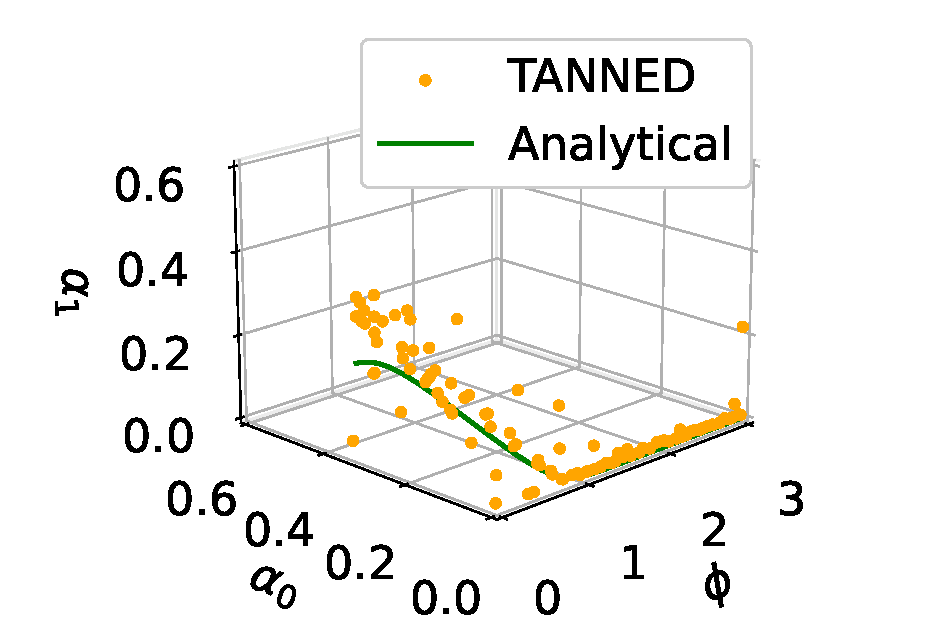
\includegraphics[width=0.7\linewidth]{figs/pop100x20_500x5g_tanned-P01-K01_01_9236fdb_22_ds.eps}
    \caption{Analytical PSNE curve for FlipIt with IE.}
    \label{fig:analytical_decision_space}
\end{figure}

\begin{figure}[h]
    \centering
    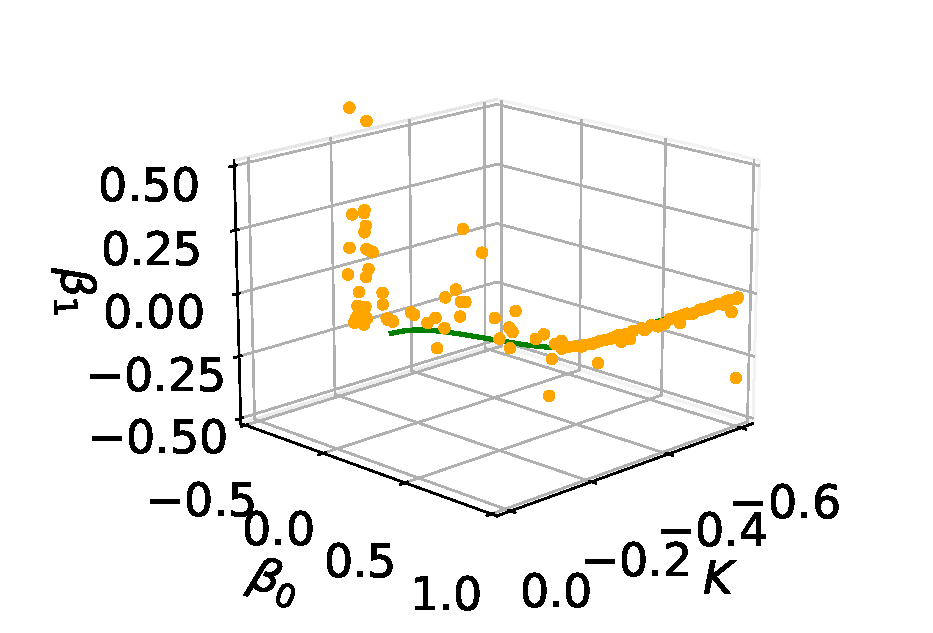
\includegraphics[width=0.7\linewidth]{figs/pop100x20_500x5g_tanned-P01-K01_01_9236fdb_22_os.eps}
    \caption{Payoff for the PSNE curve.}
    \label{fig:analytical_objective_space}
\end{figure}

%----------------------------------------------------------------------------------------

\section{Proposed Approach}
\label{algorithm}

In the decision-variable CoEA by Leite et al. \cite{leite2024cec}, a fitness composed of a single scalar was computed for each decision-variable value, and a simple proportional selection scheme was used to select the best values during evolution.
In the MOEA grid-based framework \cite{leite2024jpnsec} and the single-PSNE CoEA approach \cite{leite2025gecco} by the same authors, MOEAs were used to solve player problems as part of the process of finding PSNE, guided by the Pareto-dominance relation.

What all of these approaches have in common is the use of traditional ranking concepts to drive the search, be this search for a single- or multi-objective optimization as a part of the PSNE search, or be it directly for the PSNE search itself.
For example, for single-objective optimization, solutions are ranked based simply on their fitness values: better fitness means better rank.
When the non-dominated sorting concept present in NSGA-II \cite{Deb_2002} was used, the rank is computed based on traditional Pareto-dominance between solutions.
In any case, better-ranked solutions are prioritized in the survival selection and the subsequent parent selection.
That is to say that the ranks reflect the immediate relations between the solutions in the generation in terms of fitness, and this (instantaneous) status drives the evolutionary process.

In the proposed Genetic Algorithm (GA), each individual in the population consists of a complete strategy profile, i.e., a concatenation of decision-variable values for all players in the game.
Each individual represents a \textit{candidate PSNE}, or, in other words, a PSNE estimate.
In this sense, the fitness function must evaluate how close an individual is to being a true PSNE.

Leite et al. \cite{leite2024jpnsec} define the Opponent Strategy Profile (OSP) for a given player as the strategy profile composed of the decision-variable values of all other players except the given player.
Each player's Best Response Decision Variable (BRDV) is defined as the tuple of decision-variable values that maximize the player's payoff for a given OSP.
To evaluate the fitness for each candidate, we spawn one EA per candidate and per player in the game.
Each EA is fed the OSP defined by the other players' decision-variable values in the candidate, and tasked with finding the BRDVs for the corresponding player.
We use a single-objective EA to solve each single-objective-player problem, and an MOEA for multi-objective players.
For example, for a game with three players, each with a single decision variable, a candidate with genotype (2.5, 1.0, 4.2) will spawn three EAs:
\begin{itemize}
  \item Player 1's EA has an OSP where player 2's decision variable is 1.0 and player 3's decision variable is 4.2.
  \item Player 2's EA has an OSP where player 1's decision variable is 2.5 and player 3's decision variable is 4.2.
  \item Player 3's EA has an OSP where player 1's decision variable is 2.5 and player 2's decision variable is 1.0.
\end{itemize}

In these situations, from \cite{leite2024jpnsec}, we know that a strategy profile is a true PSNE if each player's strategy is an exact BRDV for the OSP defined by the other players' BRDVs simultaneously.
In other words, assuming ``ideal EAs''\footnote{We call an ``ideal EA'' one that finds the exact Pareto front with absolute accuracy and full diversity.}, in order for an individual to be a \textit{true PSNE}, for each player, the distance between the player's strategy and one of this player's BRDVs must be zero.
With non-ideal EAs, this distance may not be exactly zero even if the candidate \textit{is} a true PSNE, due to the fact that real-world EAs have a finite population size (and thus \textit{the} perfect BRDV may not be present in the population) and a finite number of generations (and thus the population may not have converged to the true Pareto front yet).
Nonetheless, the closer this distance is to zero, the better the candidate PSNE is.
To this end, we define the \textit{player error} as the distance between the player's decision-variable value in the candidate PSNE and the closest BRDV found by the corresponding player's EA for the OSP built from the other players' decision-variable values in the same candidate.
Finally, we define the \textit{total error} of an individual as the sum of the player errors.

The proposed flow is illustrated in Fig.~\ref{fig:tanned:architecture}, where it is compared to NSGA-II.
First, the population of random PSNE estimates is initialized.
For each individual, we spawn one EA per player, setting the OSP according to the individual's genotype.
Right after initialization, we run each EA for a small, fixed number of generations, to get an initial approximation of the BRDVs for each player.
Then, we compute the total error for each individual in the population.

\begin{figure*}[h]
  \centering
  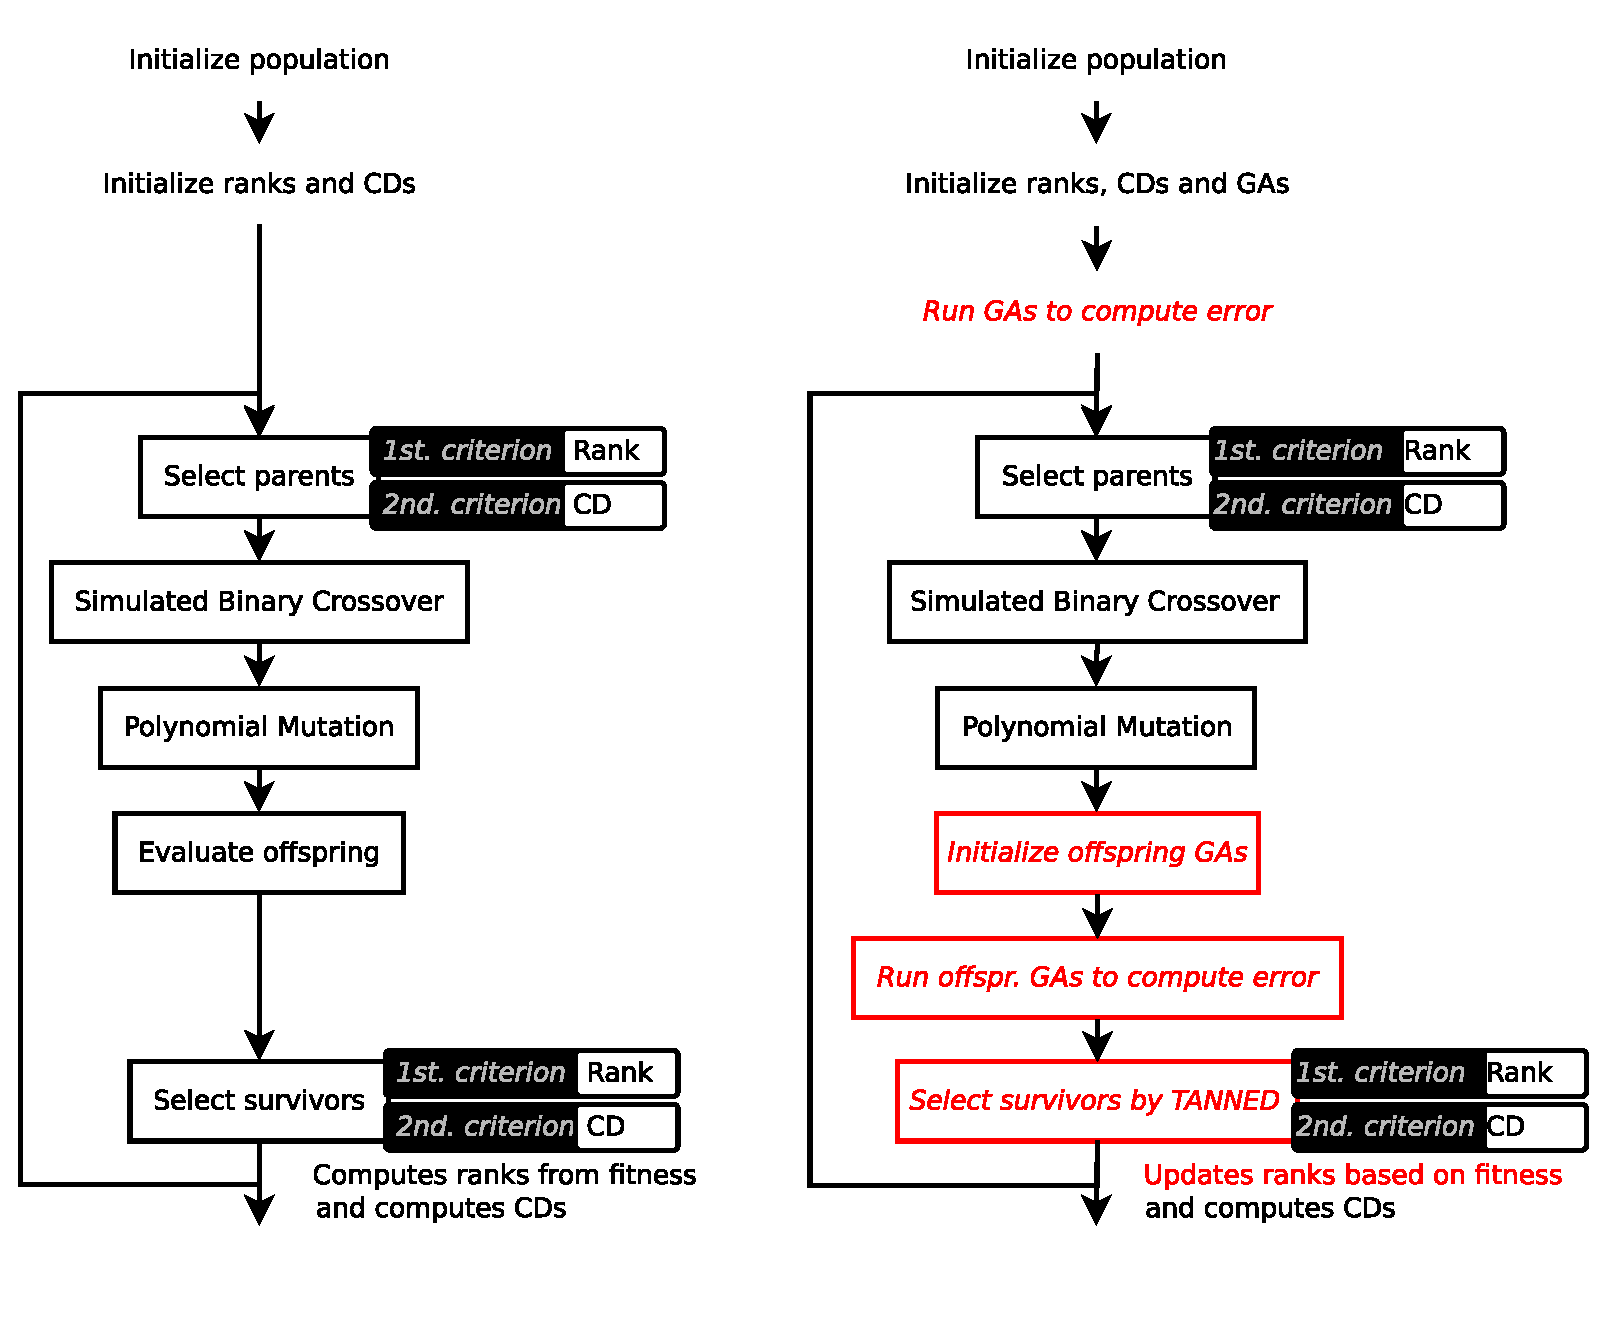
\includegraphics[width=0.8\textwidth]{./figs/flowchart_mane.eps}
  \caption{Comparison between the flow of NSGA-II (left) and the proposed algorithm (right).}
  \label{fig:tanned:architecture}
\end{figure*}

The evolutionary loop that follows selects parents based on ranks computed using a novel procedure (discussed in the next paragraph).
It then applies crossover and mutation to generate offspring, then spawns EAs to evaluate them similarly to what was done for the parents -- however, instead of initializing the EAs from scratch, we \textit{warm-start} them with the final populations from the nearest individual's EAs.
To the effect of finding the nearest individual, we compute Manhattan distances between individuals' genotypes (that is, Manhattan distances in the decision space).
Ultimately, we compute the total error for each offspring individual.
Finally, parents and offspring are combined, and the best individuals are selected using ranks produced by the following procedure.

In contrast to traditional ranking concepts, which are based on instantaneous relations between individuals in terms of fitness values (e.g., traditional Pareto-dominance), we propose a new ranking concept called TANNED.
While traditional ranking concepts leverage \textit{a priori} knowledge on the topology of the ideal solution set (e.g., the trade-off in objective space in multi-objective optimization problems), these schemes are less adequate in cases where no assumptions can be made about either the decision or the objective space.
In our case, since the objective space was reduced to an aggregate error value, the ideal solution set spans only a single point at coordinate zero (i.e., zero error).
However, this ideal set can be reached with either diverse or similar/equal individuals in decision space, meaning that if no care is taken, the search may converge to a single point in decision space.
The idea behind TANNED is to leverage information from previous generations to counteract the lack of assumptions about the topology of the ideal solution set, but still encourage diversity by avoiding a hyper-focus on optimizing fitness values alone.
This is to say that the rank of an individual is not only based on its static, immutable fitness value (the total error), but also on how this individual interacts with neighboring individuals throughout the generations.

Simply put, TANNED brings spatial information from decision space into the primary selection criterion, while still using fitness values to drive the search towards better solutions.
TANNED assumes only that there is a metric of fitness for individuals (in our case, the total error).
At initialization time, all individuals (which are all random at this point) are assigned the rank of zero.
Then, as offspring are produced at each generation, the fitness relations between offspring and parents are used to update the ranks of individuals.
More specifically, the survival selection flow with TANNED is as follows:
\begin{enumerate}
    \item Initialize offspring ranks to zero.
    \item Initialize a rank-patch vector to zero for all parents (i.e., current population individuals).
    \item Add one to the rank-patch of each of the $P$ worst-fitness parents
    \item For each offspring, find the $K$ nearest parents of the offspring in decision space, then:
    \begin{itemize}
        \item If the offspring's fitness is better than that of all neighboring parents, the offspring rank remains at zero
        \item If the offspring's fitness is worse than any neighboring parent, the offspring rank is updated to the rank of the neighboring parent with the worst fitness, plus one
        \item Every neighboring parent that has worse fitness than the offspring has its rank patched by one
    \end{itemize}
    \item Apply the rank-patch to all parents (i.e., add the rank-patch value to each parent's rank)
    \item Select the best individuals primarily by rank similarly to NSGA-II selection: add all elements from the lowest rank to the next generation's population until no more ranks can be added without exceeding the population size; then, select the remaining individuals from the next rank using CD (secondary criterion).
\end{enumerate}

The random initialization of individuals at the beginning of the search produces a diverse population with a wide range of fitness values.
GAs naturally tend to produce offspring that are similar to their parents in decision space, meaning that even very isolated individuals will be likely to have neighbors in subsequent generations as long as they have a reasonable rank.
At each generation, the worst-fitness individuals are penalized regardless of their neighborhood or rank, meaning that it is highly likely that individuals of low fitness (even isolated ones) will be eventually removed from the population and, until then, will have a reduced chance of being selected as parents.
An offspring that is worse than its neighbors is likely to have been produced in a well-explored region in decision space, thus they are penalized by being assigned a rank worse than that of their worst-fitness neighbor.
An offspring that is better than all of its neighbors is a better representative of its region in decision space, thus starting it with rank zero and penalizing the dominated neighbor encourages the replacement of the surviving/reproducing individuals in the region.

Diversity is encouraged not only by the use of CD as a secondary criterion, but also by the fact that individuals in crowded regions are more likely to being dominated them in early generations, but less likely to produce offspring that can survive/reproduce later in later generations, when the population has already a better quality overall.
Additionally, isolated individuals with excellent fitness shall be born with rank zero (when better than all neighbors), and must not suffer from rank-patching penalties even by neighboring offspring -- first because of the smaller likelihood of an offspring being generated nearby, and second because of the reduced chance of being dominated even when an offspring appears.

%----------------------------------------------------------------------------------------

\section{Experimental Setup}
\label{methodology}

To evaluate the performance of the proposed TANNED approach, we ran experiments on FlipIt with IE, the same benchmark game used in \cite{leite2024cec}, \cite{leite2024jpnsec} and \cite{leite2025gecco}.
The population size was set to 100 individuals (PSNE candidates).
Inner player EA's population size was set to 20 individuals (BRDV candidates).
Each player EA was run for 5 generations per evaluation.
The number of generations for the main GA was set to 500.
The number of nearest neighbors $K$ used in TANNED varied between 0 and 3.
The number of worst-fitness parents $P$ to be penalized at each generation was set to 10.

Two metrics were used.
GD \cite{lamont1999GD} is frequently used in evolutionary computation to measure the average distance from the estimations to the true Pareto-front.
IGD \cite{coello2004IGD} is another frequently used performance indicator that measures the opposite: the average distance from a sample of points of the true Pareto front to the generated estimations.
In our case, the distances are measured between the PSNE estimations and a sample of 200 points from the analytical PSNE curve (not the Pareto front).
Thus, from now on, we refer to our usage of these metrics as GDe and IGDe, respectively, to avoid confusion with their traditional use in multi-objective optimization.
GDe is a measure of accuracy, while the IGDe is a metric of both accuracy and diversity.

%----------------------------------------------------------------------------------------

\section{Results and Discussion}
\label{results}

The results obtained with the TANNED approach are presented in Fig.~\ref{fig:tanned:results}, where they are compared to those obtained with the decision-variable CoEA \cite{leite2024cec} and the MOEA-grid approach \cite{leite2024jpnsec}.
For the reference approaches, typical ranges of results are shown as dashed lines for comparison.
As for the TANNED approach, results for different values of $K$ and $P$ are shown; for clarity of presentation, only results for $P \neq 0$ and $K \neq 0$ are shown at this point, since the cases with $K=0$ or $P=0$ reduce to simpler versions of the proposed approach (i.e., no neighborhood consideration or no worst-fitness penalization, respectively) and have a distinctively worse performance.

\begin{figure*}[htpb]
    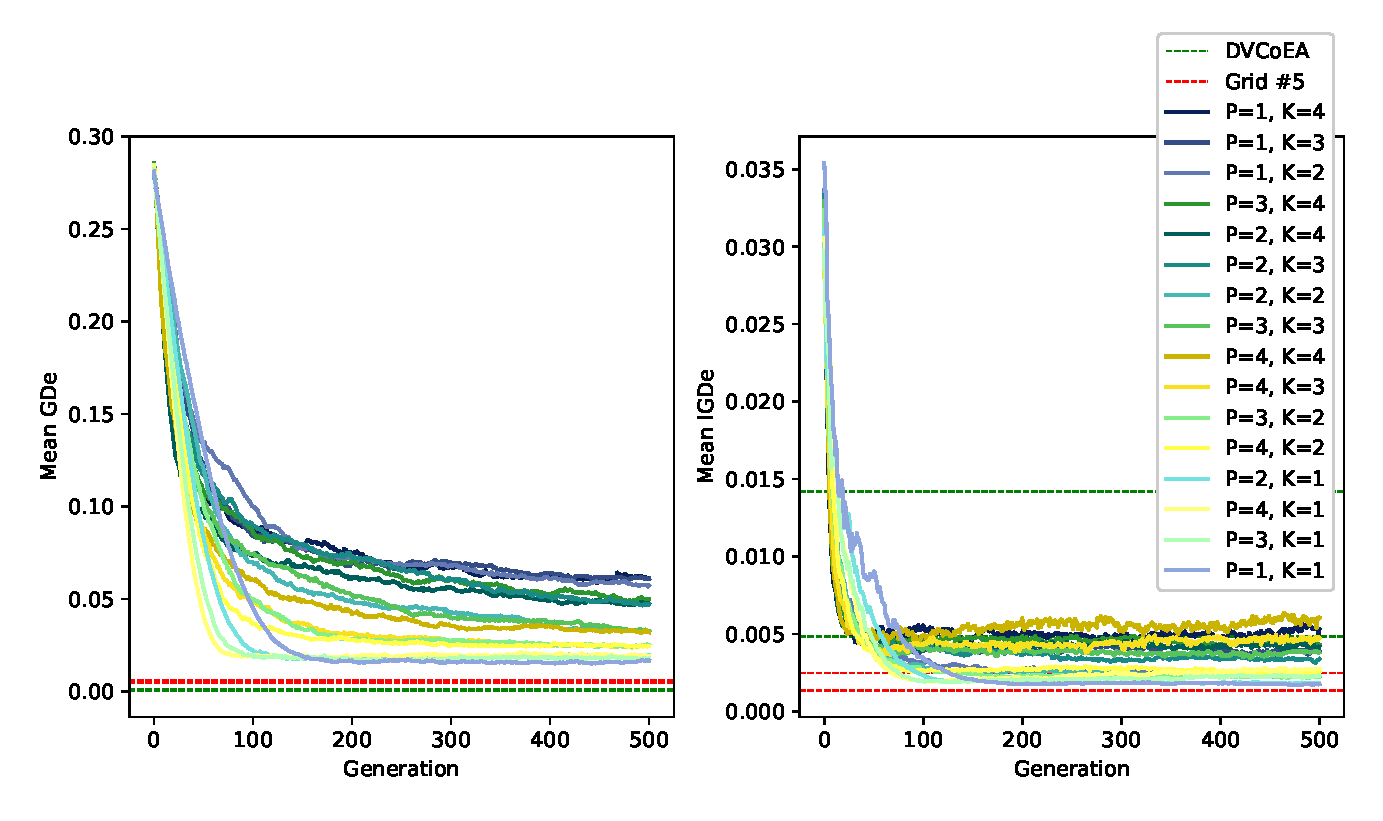
\includegraphics[width=.80\textwidth]{./figs/mane_non_zero_K_P.eps}
    \caption{Mean GDe and IGDe over generations for the TANNED approach, for runs with different values of $K \neq 0$ and $P \neq 0$; the interquartile ranges for previous approaches \cite{leite2024cec} \cite{leite2024jpnsec} are shown as dashed lines.}
    \label{fig:tanned:results}
\end{figure*}

The order of the legends is the same as that of the mean GDe at the last generation, from worst (top) to best (bottom).
As can be seen, when $K=1$, both $P=1$ and $P=2$ have a good performance.
While both reference approaches typically exhibit excellent GDe (i.e., accuracy), \cite{leite2024cec} presents a wide range of values for IGDe (i.e., accuracy and diversity), indicating that the solutions found can either be diverse or concentrated in small regions of the decision space.
\cite{leite2024jpnsec}, on the other hand, presents a range of IGDe values comparable to that of TANNED, but with an average execution time of 838.9 seconds per run, which is significantly higher than that of TANNED (257.6 seconds).
For reference, the average execution time per run of \cite{leite2024cec} was approximately 201.9 seconds.
However, it is worth noting that, as is apparent in Fig.~\ref{fig:tanned:results}, on average, the best-performing configurations of TANNED are able to reach convergence in less than 200 generations, suggesting that further reductions in execution time are possible with appropriate parameter tuning.

To allow a better understanding of the influence of parameters $K$ and $P$ on the performance of TANNED, Fig.~\ref{fig:tanned:fixed_K} presents results for five fixed values of $K$ and varying values of $P$.
As can be seen, for $K=0$, the performance is generally poor, regardless of the value of $P$.
Similarly, whenever $P=0$, the performance is poor.
This indicated that both the worst-fitness penalization and the neighborhood consideration are essential for the success of TANNED.
By turning the neighborhood off, the algorithm always creates offspring with rank zero, and only penalizes the $P$ worst-fitness parents of each generation.
When $K=1$, the performance is generally good (except for $P=0$), with most configurations rivaling typical performances of \cite{leite2024jpnsec} in terms of IGDe.
$P=1$ is the best configuration by both GDe and IGDe for all generations after approximately generation 200, when configurations with other $P$ values start to lose diversity -- possibly due to all individuals having zero rank, thus summarily eliminating individuals purely based on error alone.
For $K \geq 2$, IGDe performance degrades and even GDe seems to take longer to converge, likely indicating problems with the fitness of the solutions.
It can be concluded that the best configuration for TANNED in this problem is $K=1$ and $P=1$.


\begin{figure}[p]
  \centering
  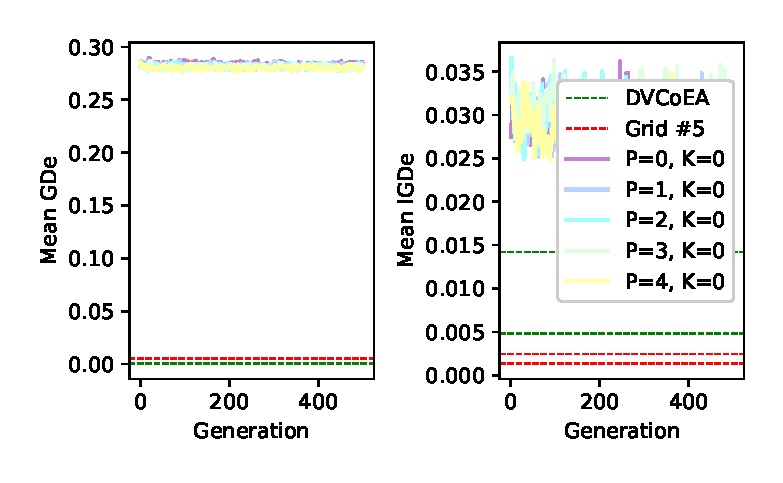
\includegraphics[width=0.94\columnwidth]{figs/mane_K_0.eps}
  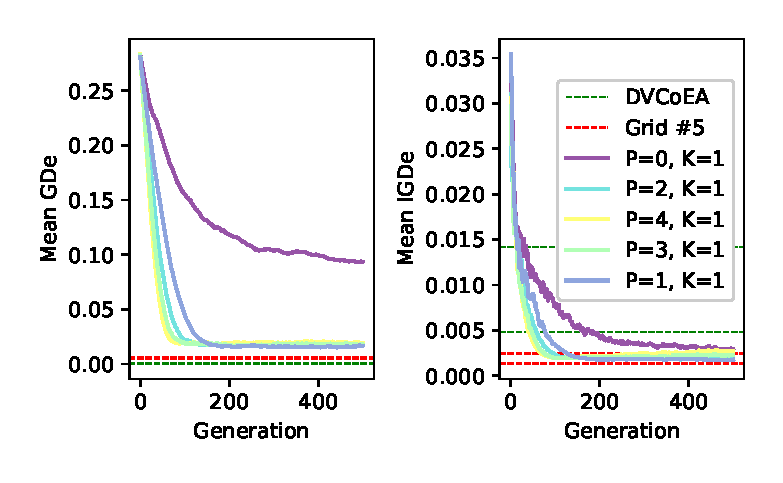
\includegraphics[width=0.94\columnwidth]{figs/mane_K_1.eps}
  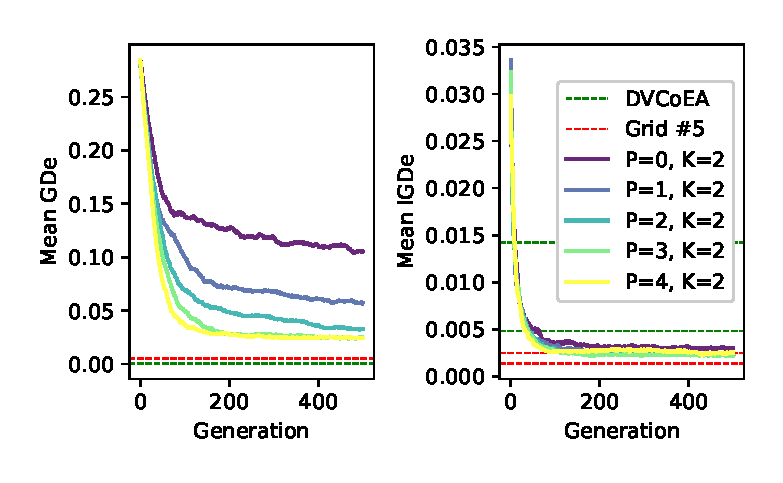
\includegraphics[width=0.94\columnwidth]{figs/mane_K_2.eps}
  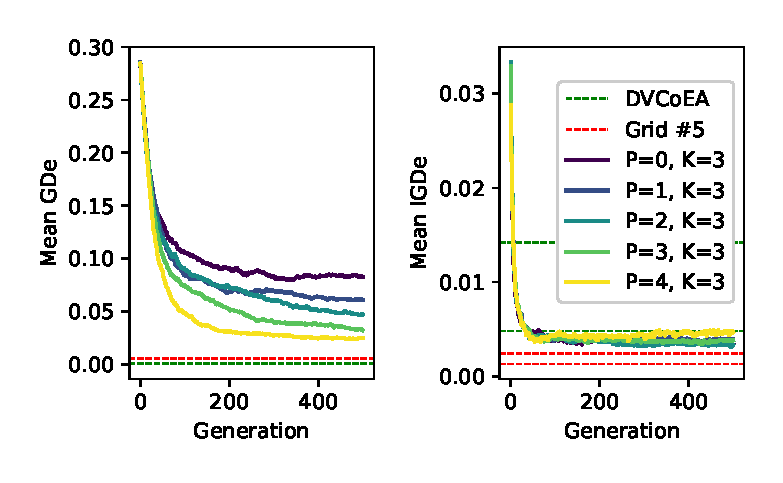
\includegraphics[width=0.94\columnwidth]{figs/mane_K_3.eps}
  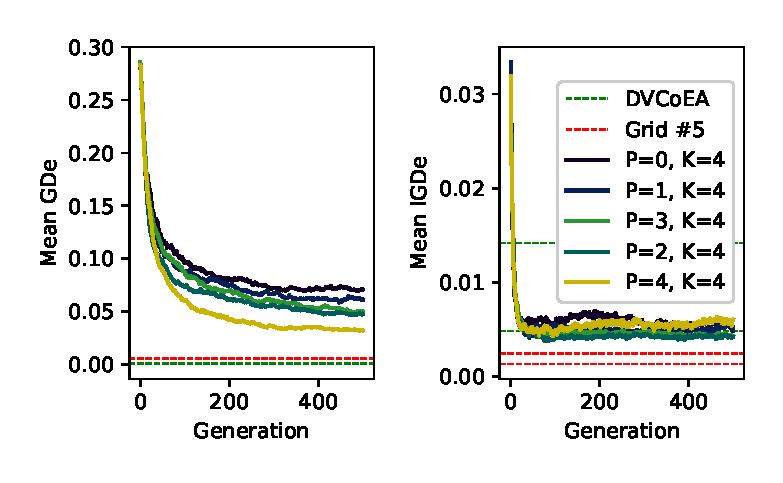
\includegraphics[width=0.94\columnwidth]{figs/mane_K_4.eps}
  \caption{Results for varying $P$ values: every row has a different fixed $K$.}
  \label{fig:tanned:fixed_K}
\end{figure}

%----------------------------------------------------------------------------------------

\section{Conclusions and Future Work}
\label{conclusions}

In this work, we presented a new GA approach for finding PSNE in multi-objective games, leveraging a novel non-instantaneous dominance concept called TANNED to guide the search.
The proposed approach was experimentally evaluated with simultaneous continuous games on the same molds of previous works.
Standard GAs were used as inner player solvers to find BRDVs for each player given the OSPs defined by candidate PSNE individuals.

While the proposed approach underperforms previous methods in terms of GDe, it rivals the best results in the literature in terms of IGDe, suggesting that it is able to find a much more diverse set of PSNE estimates.
It also shows potential to be the best performing in terms of execution times.
The architecture of the proposed approach is simpler and less hardware intensive than existing approaches, and is flexible enough to allow the use of different inner EAs for solving player problems, as well as different genetic operators for the main GA.
In future work, further improvements in the algorithm and its parameters will be explored.

\bibliographystyle{plain}
\bibliography{symposium}

%------------------------------------------------------------------------------
\end{document}
